\documentclass[a4paper,12pt]{report}

% polyglossia should go first!
\usepackage{polyglossia} % multi-language support
\setmainlanguage{russian}
\setotherlanguage{english}

\usepackage{amsmath} % math symbols, new environments and stuff
\usepackage{unicode-math} % for changing math font and unicode symbols
\usepackage[style=english]{csquotes} % fancy quoting
\usepackage{microtype} % for better font rendering
\usepackage{hyperref} % for refs and URLs
\usepackage{graphicx} % for images (and title page)
\usepackage{geometry} % for margins in title page
\usepackage{tabu} % for tabulars (and title page)
\usepackage{placeins} % for float barriers
\usepackage{titlesec} % for section break hooks
\usepackage{listings} % for listings 
\usepackage{upquote} % for good-looking quotes in source code (used for custom languages)
\usepackage{xcolor} % colors!
\usepackage{enumitem} % for unboxed description labels (long ones)
\usepackage{caption}

\defaultfontfeatures{Mapping=tex-text} % for converting "--" and "---"
\setmainfont{CMU Serif}
\setsansfont{CMU Sans Serif}
\setmonofont{CMU Typewriter Text}
\setmathfont{XITS Math}
\MakeOuterQuote{"} % enable auto-quotation

% new page and barrier after section, also phantom section after clearpage for
% hyperref to get right page.
% clearpage also outputs all active floats:
\newcommand{\sectionbreak}{\phantomsection}
\newcommand{\subsectionbreak}{\FloatBarrier}
\renewcommand{\thesection}{\arabic{section}} % no chapters
\numberwithin{equation}{section}
%\usetikzlibrary{shapes,arrows,trees}

\newcommand{\itemtt}[1][]{\item[\texttt{#1}:]} % tt-ed items (for protocol descriptions)

\definecolor{bluekeywords}{rgb}{0.13,0.13,1}
\definecolor{greencomments}{rgb}{0,0.5,0}
\definecolor{turqusnumbers}{rgb}{0.17,0.57,0.69}
\definecolor{redstrings}{rgb}{0.5,0,0}
\setmonofont{Consolas} %to be used with XeLaTeX or LuaLaTeX
\definecolor{bluekeywords}{rgb}{0,0,1}
\definecolor{greencomments}{rgb}{0,0.5,0}
\definecolor{redstrings}{rgb}{0.64,0.08,0.08}
\definecolor{xmlcomments}{rgb}{0.5,0.5,0.5}
\definecolor{types}{rgb}{0.17,0.57,0.68}

\lstset{language=[Sharp]C,
captionpos=b,
%numbers=left, %Nummerierung
%numberstyle=\tiny, % kleine Zeilennummern
frame=lines, % Oberhalb und unterhalb des Listings ist eine Linie
showspaces=false,
showtabs=false,
breaklines=true,
showstringspaces=false,
breakatwhitespace=true,
escapeinside={(*@}{@*)},
commentstyle=\color{greencomments},
morekeywords={partial, var, value, get, set},
keywordstyle=\color{bluekeywords},
stringstyle=\color{redstrings},
basicstyle=\ttfamily\small,
}

\lstset{
  numbers=left,
  numberstyle=\scriptsize,
  basicstyle=\ttfamily\scriptsize,
  columns=fullflexible,
  keepspaces, % for spaces in unicode text!
  captionpos=b
}
\renewcommand{\lstlistingname}{Листинг}

\date{\today}

\makeatletter
\let\thetitle\@title
\let\theauthor\@author
\let\thedate\@date
\makeatother

\begin{document}
\section{Глоссарий}
В настоящем документе используются следующие понятия:
\begin{itemize}
  \item пользователь -- человек, формирующий задание комплексу на проведение некоего расчёта;
  \item задача -- программа научно--прикладного характера, предоставленная в виде исполняемого файла;
  \item расчёт -- процесс выполнения задачи, результатом которого являются некие файлы (зависящие от задачи), содержащие результаты его работы. Подразумевается, что расчёт занимает значительное (от нескольких часов и до нескольких дней) время;
  \item пользовательский интерфейс, ПИ -- интерфейс, используемый для постановки задач комплексу и управления ходом их расчётов;
  \item база данных, БД -- выделенный сервер или программный компонент, отвечающий за хранение и доступ к данным;
  \item персональный компьютер, ПК -- электронно--вычислительная машина архитектуры IBM PC;
  \item вычисляющий компьютер, ВК -- ПК с установленным ПО, обеспечивающим взаимодействие данного ПК с комплексом и проведение расчётов на данном ПК;
  \item СОА -- ``сервис-ориентированная архитектура(SOA)'', подход к разработке программного обеспечения на основе слабосвязанных компонентов, взаимодействующих посредством стандартизованных интерфейсов;
  \item сервер -- объект клиент -- серверного взаимодействия, осуществляющий обслуживание клиентов
  \item клиент -- объект клиент -- серверного взаимодействия, инициирующий запрос серверу
  \item бекенд -- сервер, элемент декомпозии СОА, отвечающий за выполнение определенной подзадачи(работы с определенным типом данных, балансировку и т.д.);
  \item фронтенд -- сервер, элемент декомпозии СОА, отвечающий за перенаправление запросов бекендам и предоставление ПИ и/или интерфейса приложения.
\end{itemize}

\section{Введение}

Настоящее техническое задание распространяется на разработку программного комплекса, выполняющего задачи распределения вычислительных мощностей персональных компьютеров в рамках исследовательских коллективов. Разрабатываемый комплекс позволит задействовать простаивающие вычислительные ресурсы под расчёты научных задач. Техническое задание выполняется в соответствии со стандартом ГОСТ 34.602--89 "Техническое задание на создание автоматизированной системы".

В ходе исследовательских работ в разных областях у членов научно--исследовательских и технических коллективов часто возникают задачи расчёта небольших программ, призванных проверить какую--либо гипотезу. 
Время работы подобных программ, несмотря на их простоту, может достигать нескольких часов, и в рамках коллектива часта ситуация, когда в любой момент времени кто--либо проводит какие--либо расчёты. 
В то же время, для каждого конкретного исследователя время расчёта подобных программ не занимает всё доступное. 
Част режим работы, в котором конкретный сотрудник несколько дней планирует вычислительный эксперимент, после чего ему необходимо поставить его на выполнение на несколько часов. 
В эти несколько часов его компьютер находится под высокой нагрузкой; однако во время нескольких дней планирования он по большей части простаивает.

В связи с этим возникла необходимость реализации программного комплекса, позволяющего исследователям в рамках коллектива загружать вычислительными задачами компьютеры друг друга.
Комплекс должен быть прост в обращении и не требовать особой доработки программного обеспечения вычислительных экспериментов для их расчёта.

\clearpage
\section{Существующие аналоги}

Подобные системы разрабатываются с 1994 года, и в общем случае их называют системами "добровольных вычислений".
Среди программного обеспечения, используемого для организации таких вычислений, наиболее распространены системы XtremWeb, Xgrid, Grid MP и BOINC.
Все подобные программы работают по одному и тому же принципу -- пользователь в заданном формате передаёт системе свою программу; система отправляет эту задачу на выполнение какому-либо из вычислительных узлов, получает ответ и отдаёт его пользователю.

Xgrid -- технология, разработанная компанией Apple, позволяющая объединять группу компьютеров в виртуальный суперкомпьютер для проведения распределённых вычислений. 
Из преимуществ данной системы можно выделить наличие предустановленных клиентов на компьютерах под управлением MAC OS X; однако её недостатки весьма существенны -- во-первых, существует только реализация для MAC OS X; во-вторых, для доступа к каким-либо функциям комплекса, кроме просто однопоточного запуска программы, исполняемая программа должна быть специально спроектирована с учётом особенностей системы и только на языке Objective-C.

Grid MP -- технология, разработанная компанией Univa. Символы MP в названии не имеют официальной расшифровки. 
Предоставляет web API для манипулирования объектами системы, что позволяет вести разработку для комплекса на практически любом языке программирования, но в то же время требует разработки программ специально под комплекс.

BOINC -- открытая программная платформа университета Беркли для GRID вычислений. 
Обеспечивает валидацию вычислений за счёт избыточности, отслеживание конкретного вклада пользователей в расчёты, управление участием в различных экспериментах; однако рассчитан на огромные по масштабам проекты (тысячи и сотни тысяч вычислителей; наиболее крупные проекты насчитывают до 15 миллионов участников). 
В связи с этим, процесс настройки проекта занимает значительное время.

TORQUE -- (Terascale Open-Source Resource and QUEue Manager) -- менеджер распределенных ресурсов для вычислительных кластеров из машин под управлением Linux и других Unix-подобных операционных систем. Существует порт под Windows.

Таким образом, из известных систем подобного рода ни одна не занимает целевую нишу ввиду следующих особенностей: 
\begin{itemize}
  \item Xgrid -- поддерживает только MAC OS системы, исполняемая программа должна быть написана специально для работы с данной системой;
  \item Grid MP -- коммерческий продукт, данных о ценах нет в наличии; исполняемая программа должна быть написана специально для работы с данной системой;
  \item BOINC -- избыточная дла поставленной задачи функциональность, исполняемые прикладные программы должны сильно дорабатываться для совместимости с проектом;
  \item TORQUE -- система не предусматривает механизм деградации функциональности.
\end{itemize}

\section{Основание для разработки}
Программа разрабатывается на основе учебного плана кафедры "Программное обеспечение ЭВМ и информационные технологии".

\section{Назначение разработки}
Основным назначением комплекса является утилизация простаивающих вычислительных мощностей в рамках исследовательских коллективов.

\section{Требования к программному изделию}
\subsection{Функциональные требования}
Комплекс должен обеспечивать возможность выполнения следующих функций:
\subsubsection{С точки зрения пользователя, устанавливающего задачу}
\begin{itemize}
  \item регистрация пользователя в сети;
  \item постановка произвольной задачи с указанием минимальных параметров технических и программных средств, необходимых задаче;
  \item отслеживание состояния выполнения задачи;
  \item досрочная остановка выполнения задачи;
  \item просмотр отчёта о завершении задачи или всех таких отчётов в случае, если выполнение задачи дублировалось на разных компьютерах;
\end{itemize}

\subsubsection{С точки зрения пользователя, предоставляющего вычислительные мощности}
\begin{itemize}
  \item регистрация компьютера в сети;
  \item начало предоставления вычислительных мощностей;
  \item установка лимита использования процессорного времени;
  \item выключение компьютера по завершению текущего расчёта;
  \item остановка предоставления вычислительных мощностей;
\end{itemize}

\subsubsection{С точки зрения администратора}
\begin{itemize}
  \item динамическое добавление вычисляющих компьютеров в сеть и удаление их из сети должно происходить прозрачно для пользователей;
  \item наличие системы мониторинга для отслеживания состояния сети;
\end{itemize}


\subsection{Входные параметры комплекса}
В качестве входных параметров со стороны пользователя комплексу предоставляются:
\begin{itemize}
  \item исполняемый файл задачи;
  \item текстовый документ формата, выработанного в ходе разработки, содержащий: 
  \begin{enumerate}
    \item требования к аппаратному и программному обеспечению ВК;
    \item список выходных файлов задачи;
  \end{enumerate}
  \item сведения о необходимости дублирования расчёта на нескольких ВК.
\end{itemize}

Со стороны ВК в автоматическом либо ручном режиме работы комплексу предоставляются сведения о аппаратном и программном обеспечении, 
позволяющие балансировщику принимать решения о назначении задачи конкретному ВК.

\subsection{Выходные параметры комплекса}
Комплекс должен предоставлять пользователю следующую информацию:
\begin{itemize}
  \item данные о текущем статусе поставленных задач -- выполнена, выполняется, ожидает свободного ВК, приостановлена, отменена;
  \item для завершённых или частично завершённых задач -- список поступивших отчётов о завершении расчёта;
  \item данные о текущем состоянии сети -- список в данный момент подключенных ВК, данные по их активности.
\end{itemize}

\section{Сценарии функционирования системы}
\begin{itemize}
  \item Постановка задачи на исполнение
  \begin{enumerate}
    \item Пользователь осуществляет вход в ПИ со своими учётными данными
    \item Авторизованный пользователь добавляет новую задачу через ПИ, предоставляя все данные, указанные в пункте "Входные данные"
    \item Задача ставится в очередь на выполнение
    \item Система ожидает запроса от свободного ВК на получение задачи
    \item Система передаёт ВК задачу и необходимые ей данные и ожидает ответа
    \item Далее возможны варианты:
      \begin{itemize}
        \item Расчёт успешно завершается и ВК передаёт результаты расчёта системе
        \item Расчёт завершается ошибкой и ВК передаёт отчёт об ошибке системе
        \item В ходе расчёта ВК перестаёт сообщать балансировщику о ходе работы. Балансировщик ждёт сообщений от ВК в течение указанного максимального времени ожидания, и считает ВК нештатно завершившим работу. Балансировщик повторяет помещение задачи в очередь на выполнение с повышенным приоритетом. Если ВК вновь окажется в сети, переданные им результаты не будут учтены.
      \end{itemize}
  \end{enumerate}
    
  \item Просмотр статуса выполнения задачи
  \begin{enumerate}
    \item Пользователь осуществляет вход в ПИ со своими учётными данными
    \item Авторизованный пользователь выбирает одну из собственных задач через ПИ
    \item Система генерирует отчёт, содержащий информацию о статусе выполнения задачи и все полученные на данный момент отчёты о завершении расчётов, полученные от ВК
  \end{enumerate}
  
  \item Отмена исполнения задачи
  \begin{enumerate}
    \item Пользователь осуществляет вход в ПИ со своими учётными данными
    \item Авторизованный пользователь отменяет выполнение одной из собственных задач через ПИ
    \item Система помечает задачу как отменённую, и при получении следующего отчёта от ВК о статусе выполнения задачи в ответ передаёт команду остановки расчётов
  \end{enumerate}
\end{itemize}

\subsection{Требования к структуре}
Комплекс должен удовлетворять следующим требованиям:
\begin{itemize}
  \item структура системы должна следовать принципам СОА;
  \item количество качественно различных сервисов, из которых должна состоять система, должно быть не меньше 4-х;
  \item не менее 3-х сервисов(бекендов) должны быть горизонтально масштабируемыми;
  \item взаимодействие сервисов должно осуществляться по HTTP протоколу с учётом рекомендаций REST, если не доказана необходимость отказа от такого решения;
  \item отслеживание авторизационных ключей должно осуществляться отдельно выделенным сервисом;
  \item база данных комплекса должна поддерживать репликацию; 
\end{itemize}

Топология проектируемой системы представлена на рис.~\ref{fig:topology}.

\begin{figure}
    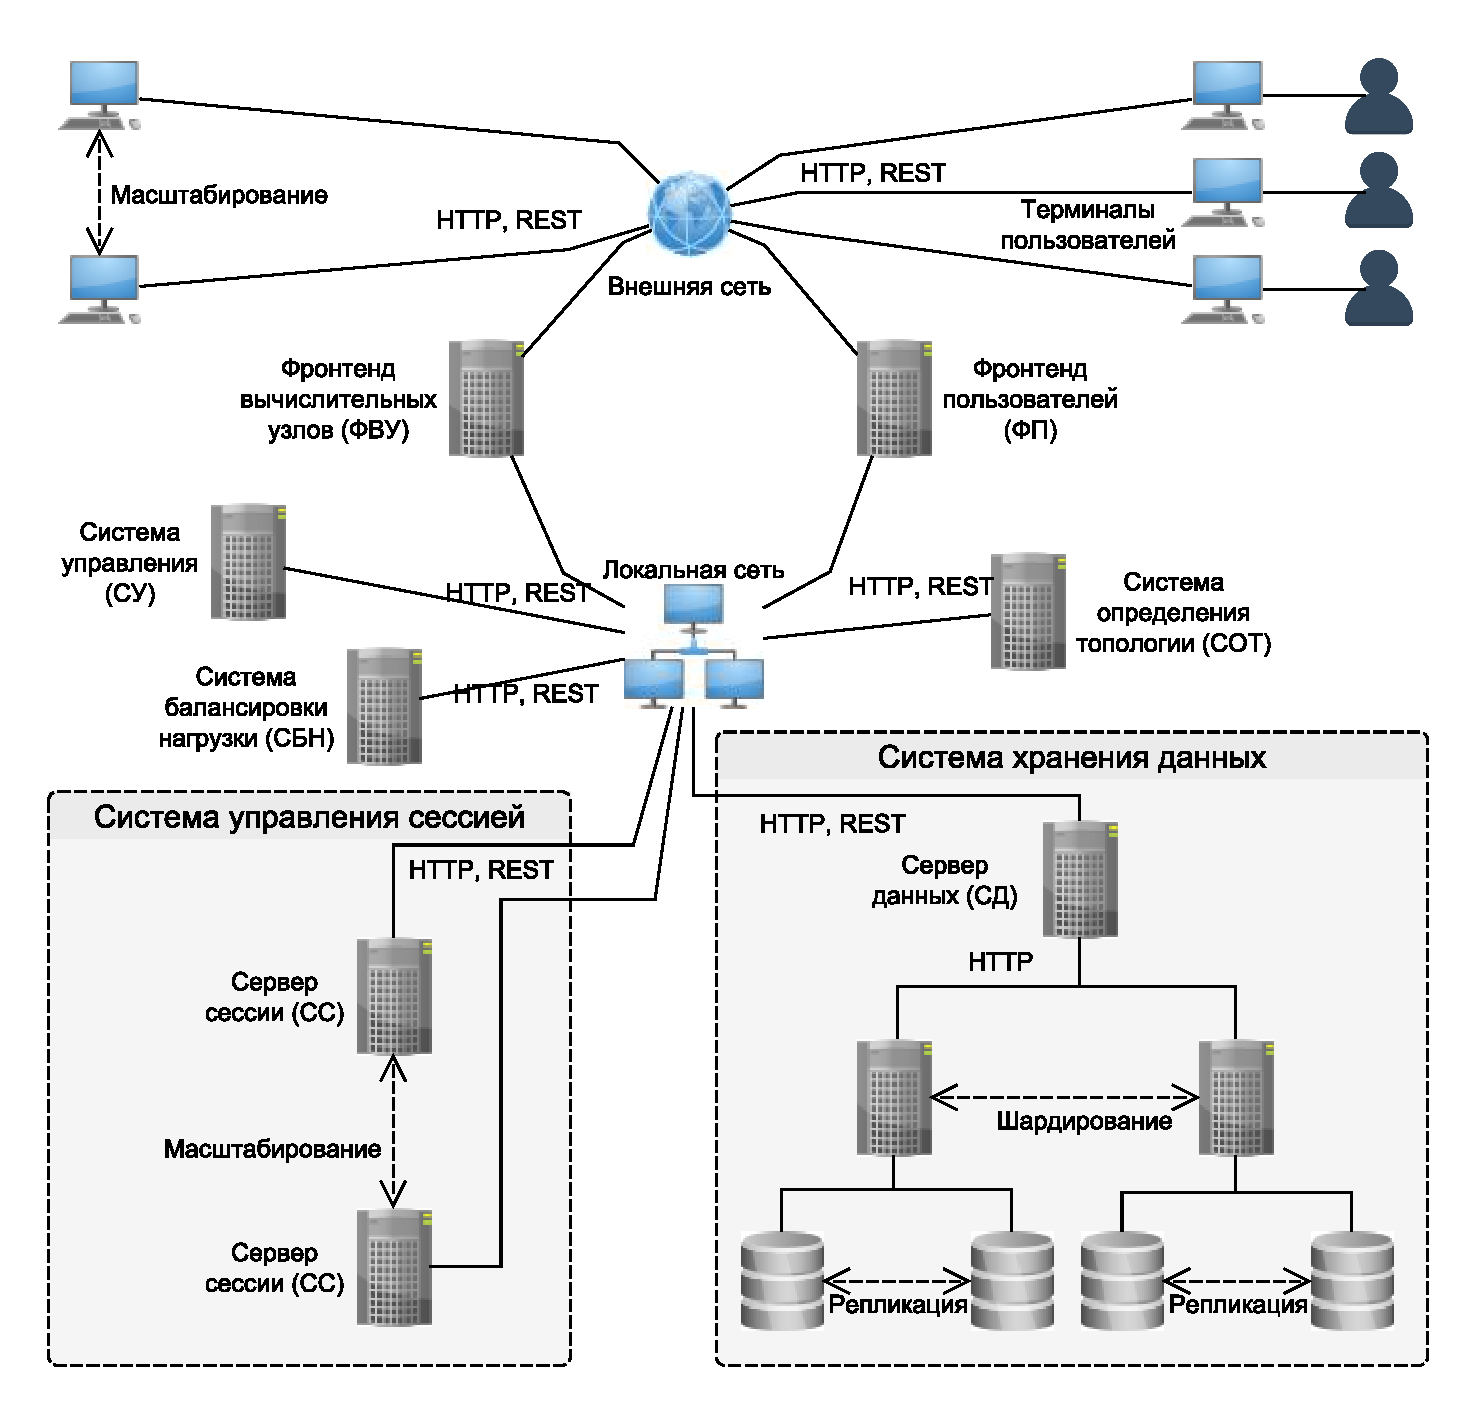
\includegraphics[width=\linewidth]{img/schema-tz.eps}
    \label{fig:topology}
    \caption{Топология проектируемой системы.}
\end{figure}

\subsubsection{Требования к системе хранения данных}
Система хранения данных (СХД) должна предоставлять запрашивающему клиенту следующий функционал:
\begin{itemize}
  \item доступ к данным внутри системы на чтение и запись
  \item шардирование БД
  \item репликацию БД
  \item абстрагирование структуры БД через REST -- API
\end{itemize}

\subsubsection{Требования к системе балансировки нагрузки}
Система балансировки нагрузки (СБН) должна предоставлять запрашивающему клиенту следующий функционал:
\begin{itemize}
  \item выдача новой задачи, требующей исполнения;
  \item приём результатов выполения задачи;
  \item приём оповещений о статусе вычисляющего узла;
\end{itemize}

Вышестоящей в иерархии взаимодействия сущности СБН должна предоставлять следующий функционал:
\begin{itemize}
  \item выполнение задач из пула поставленных задач
  \item отслеживание состояния вычислительных узлов и выполняющихся на них задач
  \item досрочная остановка выполнения задачи
\end{itemize}

\subsubsection{Требования к системе управления}
Система управления (СУ) должна предоставлять пользователю следующий функционал:
\begin{itemize}
  \item постановка задачи на исполнение;
  \item просмотр результатов выполения задач пользователя;
  \item досрочная остановка выполнения задач(и) пользователя;
  \item просмотр статуса выполнения задач пользователя;
\end{itemize}

Администратору СУ должна предоставлять функционал просмотра и управления задачами всех пользователей.

\subsubsection{Требования к системе управления сессией}
Фронтенд вычислительных узлов должен предоставлять запрашивающему клиенту следующие возможности:
\begin{itemize}
    \item валидация предоставленного клиентом ключа доступа к сети;
    \item авторизация клиента по предоставлению им корректных регистрационных данных;
    \item регистрация новых клиентов и генерация и предоставление им ключей доступа к сети;
\end{itemize}

\subsubsection{Требования к системе определения топологии}
Система определения топологии (СОТ) необходима для облегчения процесса разворачивания системы.
СОТ должна предоставлять запрашивающему клиенту следующий функционал:
\begin{itemize}
  \item клиент может уведомить СОТ о том, что он является определённым сервером с определённым именем по определённому адресу и порту;
  \item клиент может запросить у СОТ список всех зарегистрированных в ней серверов с их именами, адресами и портами;
\end{itemize}

\subsubsection{Требования к фронтенду вычислительных узлов}
Фронтенд вычислительных узлов (ФВУ) должен дублировать функционал системы балансировки нагрузки. Помимо этого, ФВУ должен, опрашивая систему управления сессией, осуществлять проверку корректности предоставленных запрашивающим узлом ключей доступа.

\subsubsection{Требования к фронтенду пользователей}
Фронтенд пользователей (ФП) должен дублировать функционал системы управления. Помимо этого, ФП должен, опрашивая систему управления сессией, осуществлять проверку корректности предоставленных запрашивающим пользователем ключей доступа.

\subsection{Требования к надежности}
Комплекс должен быть спроектирован с учётом контролируемой деградации, то есть в случае ошибки продолжать обеспечивать хотя бы часть функционала. Примеры таких ситуаций:
\begin{itemize}
  \item внезапное отключение ВК не должно приводить к "зависанию" задачи на стадии выполнения, балансировщик должен определять такие ситуации и передавать задачу другому исполнителю;
  \item внезапное завершение работы задачи не должно приводить к остановке работы ВК, он должен отправить отчёт о работе задачи балансировщику и запросить новую задачу;
  \item внезапное отключение балансировщика не должно влиять на ход расчёта задач и должно быть отражено в интерфейсе администратора;
  \item внезапное отключение сервера, осуществляющего взаимодействие с пользователем, не должно влиять на ход расчёта уже поставленных комплексу задач.
\end{itemize}

\subsection{Требования к информационной и программной совместимости}
На программное обеспечение серверных частей комплекса ограничения не накладываются.
Комплекс должен поддерживать как вычисляющие компьютеры под управлением ОС Windows (начиная с 7), так и Linux.
Желательно использование нескольких языков программирования для реализации разных сервисов.

\section{Требования к программной документации}
Программная документация должна удовлетворять следующим требованиям:
\begin{itemize}
  \item разрабатываемые программные модули должны быть самодокументированны, т.е. тексты программ должны содержать все необходимые комментарии;
  \item документация должна включать в себя отчёты о модульном, интеграционном и системном тестированиях программы
  \item документация должна включать в себя краткое руководство пользователя
\end{itemize}

\end{document}